\subsection{Extensions to the Basic Agent}
The agent design outlined in the preceding sections of this chapter addresses the problem outlined in Section \ref{subsec:ProbDescription},  following the assumptions outlined in Section \ref{subsec:initalAssumptions}. As mentioned in Section \ref{subsec:initalAssumptions}, some of these assumptions are not realistic, which we address in this section. \par

\subsubsection{Localising Multiple Targets}
The first assumption that we address is that there are either zero or one targets to be localised. In many applications, this is a very unrealistic assumption. For example, the ROCSAFE project (outlined in section \ref{sec:ROCSAFEBG}), which motivates this work, aims to apply object detection algorithms to aerial images in order to avoid the need to send a crime scene investigator into a hazardous scenario in order to verify the presence of a potential source of evidence.\note{check the above sentence is consistent with the Background} An assumption that is much more valid is that there are a maximum of $k$ unknown sources present in the search region, which addresses the general case for the ROCSAFE \note{should ROCSAFE be in italics?} project.\par

\note{May need to go into more detail here since people without a background in probability might not understand implications of high-dimensional joint distribution}
The main issue that arises when including \textit{multiple} targets in the hidden state, $X_t$, is that there is an exponential increase the dimensionality of the hidden state for each new target added. This means that maintaining an estimate of the state quickly becomes infeasible, since the run time of the forward algorithm detailed in section \ref{subsubsec:filteringDBN} is dependent on the square of the size of the joint distribution of the hidden state variables, $X_t$ and the memory requirements for maintaining the estimated state also depend on the dimensionality of the joint distribution of the hidden state. See section \ref{subsubsec:filteringDBN} for details of the filtering algorithm.


Section <reference lit review> of the literature review outlines a number of techniques that have been applied by other researchers in this domain in order to deal with the case of multiple targets. \note{maybe should leave all of this to lit. review and just outline what I did.} Related work \cite{Waharte2009CoordinatedUAVs} proposed to use an approach commonly used with occupancy grids, which is that every grid cell may or may not contain a target, independent of whether or not all other grid cells contain a target. This technique is often referred to as \textit{mapping} when the location of the agent is known. This is generally described by \citeauthor{Thrun:2005:ProbabilisticRobotics} in  \cite[P.~284]{Thrun:2005:ProbabilisticRobotics}. Rather than maintain a multinomial distribution for $TargetLocation_{t-1}$, as was the case in the work outlined in this chapter, we create a new binary random variable representing a target being present or not in each grid cell, denoted $m_i$ for $i \in \{1,...,N\}$. We denote m as the joint distribution of these random variables. The DBN that corresponds to this is shown in Figure \ref{fig:DBNWithMultipleIndependent}. The associated update rule simply 

\begin{figure}
    \centering
    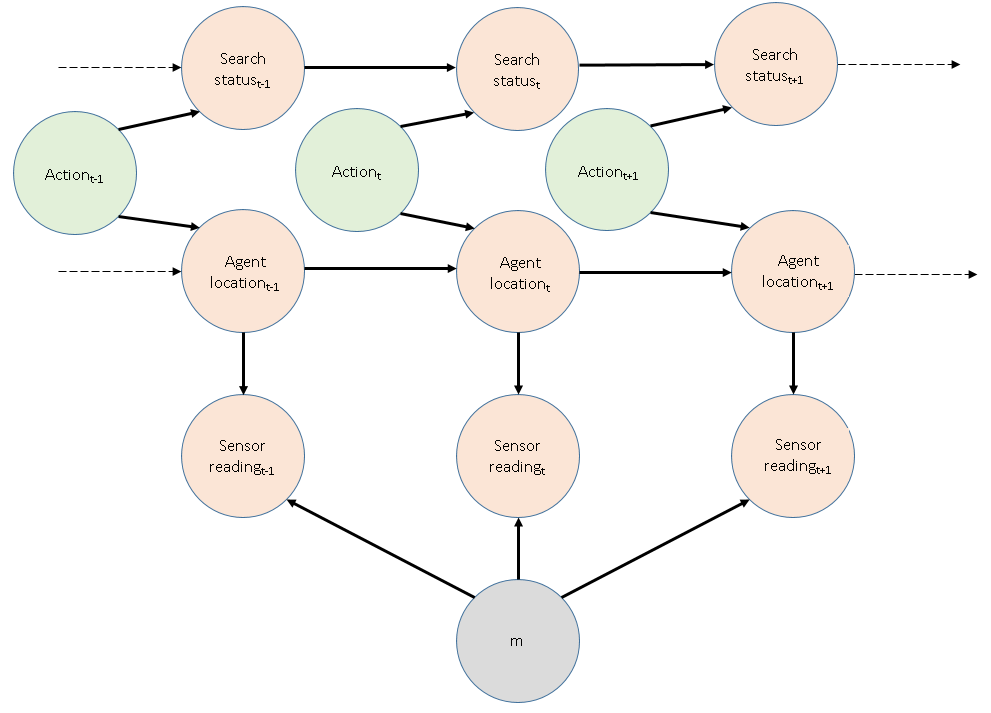
\includegraphics[width = 0.75\linewidth]{Chapters/MultiAgentTargetDetection/Figs/DBNs/DBNWithMultipleIndependentSources.png}
    \caption{The DBN which takes into account that there could be a target in each of the grid cells}
    \label{fig:DBNWithMultipleIndependent}
\end{figure}





In the case, estimating the joint distribution is not hard, since This results in a greatly simplified state estimate update equation, where the probability of the target being located in a grid cell does not change unless the observation was made in that grid cell. The major drawback of this approach is that there is no clear way to apply the SPRT, hence there is no clear way to decide when to terminate the search. 


stems from the fact that this assumption induces a simple dependence relation between grid cells, for which the update rule \ref{eqn:SearchStatus} can 


The first method, which is very commonly taken when using an approach that uses occupancy grids \cite{Elfes1989UsingNavigation}, is to assume that grid cells are indeped
